\section{Special Case Analysis}

\subsection{Definitions for Analysis}

\begin{frame}{Definitions for Analysis}
  Its an empty frame to keep latex from compiling the movie!
  % \begin{columns}[T]

  %   \column{0.5\textwidth}

  %     \only<1->{
  %       \begin{block}{Definition: 2D Stencil Interval Vertex Coloring (2DS-IVC)}<1->
  %         A problem where \( G \) is a \( 9 \)-pt \( 2D \) stencil, 
  %         composed of \( X \times Y \) vertices on a \( 2D \) grid such that two vertices \( (i, j) \) 
  %         and \( (i', j') \) are connected iff \( |i - i'| \leq 1 \) and \( |j - j'| \leq 1 \).
  %       \end{block}
  %     }
  %     \null
  %     \centering
  %     \only<2->{
  %       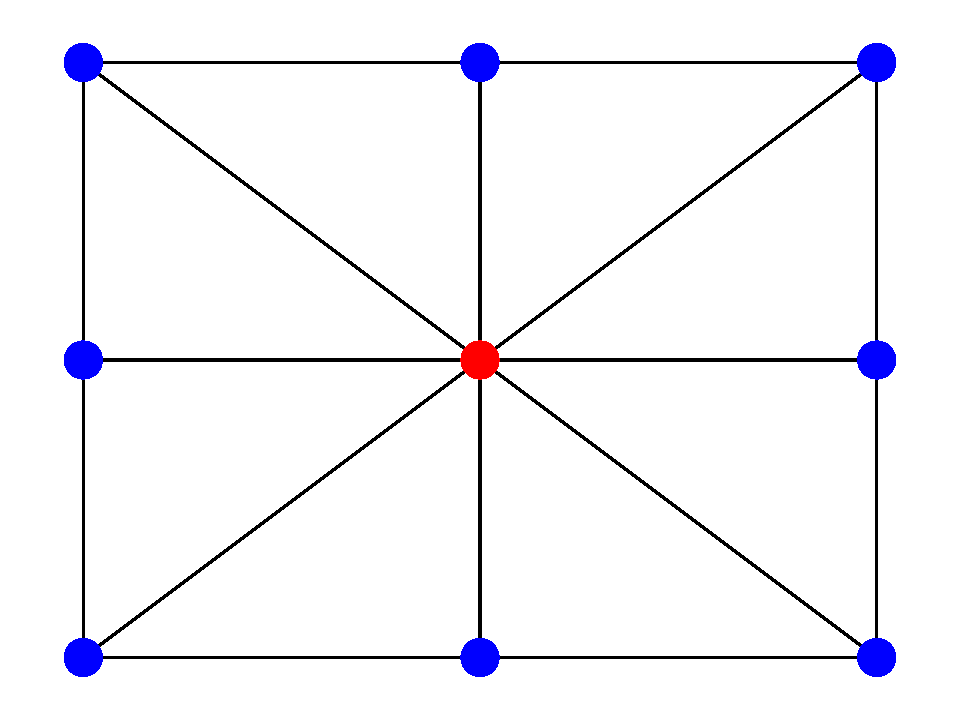
\includegraphics[width=0.5\textwidth]{figures/9pt_stencil_graph.pdf}<2->
  %     }

  %     \null
  %     \null
  %     \null
  %     \null


  %   \column{0.5\textwidth}
  %       \only<3->{
  %         \begin{block}{Definition: 3D Stencil Interval Vertex Coloring (3DS-IVC)}
  %           A problem where \( G \) is a 27-point \( 3D \) stencil, 
  %           composed of \(X \times Y \times Z\) vertices on a 3D grid such that two vertices 
  %           \( (i, j, k) \) and \( (i', j', k') \) are connected iff \( |i - i'| \leq 1 \), \( |j - j'| \leq 1 \), and
  %           \( |k - k'| \leq 1 \).
  %         \end{block}
  %       }
  %     \centering
  %     \only<4->{%
  %       \animategraphics[loop,width=0.8\textwidth, autoplay]{30}{figures/animation_27pt/output_}{0001}{180}
  %     }
  % \end{columns}
\end{frame}

\subsection{Special Cases}

\begin{frame}{Cliques $K_n$}
  \begin{theorem}<1->
    Let $G(V,E)$ be a clique $K_n$ with $n$ vertices, then  \[ \text{maxcolor}= \sum_{v \in V} w(v) \]
    is indeed an optimal coloring maxcolor* .
  \end{theorem}

  \begin{itemize}
    \item<2-> There exists such a coloring by listing vertices in descending order of weights and
    greedily allocating the color inteveral with the lowest available start(v) with $\mathcal{O}(n)$ \qed .

    \item<3-> Particularly important result since the 2D-IVC's and 3D-IVC's are composed of $K_4$'s and $K_8$'s
    respectively.

    \item<4-> Therefore any identified $K_4$ in a 2D-IVC Problem and any $K_8$ in a 3D-IVC Problem are immediately
    (lose) lower bounds on maxcolor.
  \end{itemize}
\end{frame}

\begin{frame}{Bipartite Graphs}
  \begin{Theorem}<1->
    A graph G(V,E) is Bipartite iff it contains no odd cycles. In other words: its vertices can be partitioned into
    two sets A and B, such that all edges have one endpoint in A and the other in B.
  \end{Theorem}

  \begin{itemize}
    \item<2-> All edges provide trivial lower bound: $ \text{maxcolor*} \ge  w(i) + w(j), \forall (i, j) \in E.$
    \item<3-> There exists a coloring \\ 
    $\text{maxcolor*} = \max_{(i,j) \in E} w(i) + w(j)$ in $\mathcal{O}(|E|)$. (Proof Omitted)
    \item<4-> Another important result, since the 9-pt stencil contains a Bipartite 5-pt stencil and the
    27-pt stencil constains at least a Bipartite 7-pt stencil, and all paths are Bipartite.
    \item<5-> Authors use this to construct approximation algorithms.
  \end{itemize}
\end{frame}

\begin{frame}{Odd Cycles 1}
  \begin{itemize}
    \item<1-> Graphs that are not Bipartite, contain at least one cycle of odd length.
    \null
    \item<2-> Odd cycles have optimal interval colorings that are strictly greater than the largest weight of
    any clique in the cycle.
    \null
    \item<3-> The clique with the largest weight from the cycle shown earlier would be of interval size 25, while the
    optimal coloring of the entire graph (the odd cycle) has maxcolor* = 30.
    \null
    \item<4-> Understanding of coloring of odd cycles yields new lower bounds.
  \end{itemize}
\end{frame}

\begin{frame}{Odd Cycles 2}
  
  \begin{definition}<1->
    Let maxpair be the maximal sum of any two consecutive vertices. \footnotemark
    \[ \text{maxpair} = \max_i w(i, i + 1) \]
  \end{definition}

  \begin{definition}<2->
    Let minchain3 be the minimum sum of any 3 consecutive vertices:
    \[ \text{minchain3} = \min_i w(i, i + 1, i+2) \]
  \end{definition}

  \begin{theorem}<3->
    Let G be an odd cycle, then it holds:
    \[ \text{maxcolor*} = \text{max}(\text{maxpair, minchain3}) \]
  \end{theorem}

  \footnotetext{Here G is cycle, neighbors of vertex $x$ are $x+1$ and $x-1$.}
\end{frame}

\begin{frame}{Odd Cycles 3}
  \begin{block}{Idea of Proof}<1->
    \begin{itemize}
      \item<2-> If G is an odd cycle, there is an algorithm
      that yields max(maxpair, minchain3) colors, which 
      means $\text{maxcolor*} \leq \max(\text{maxpair, minchain3})$.
      \null
      \null
      \item<3-> If G is an odd cycle, then $\text{maxcolor*} \ge \max(\text{maxpair, minchain3})$.
      \null
      \null
      \item<4-> Coinciding bounds conclude proof \cite{main_paper} $\qed$ .
      \item<5-> One can verify this for the previous example
    \end{itemize}
  \end{block}
  
  \visible<5->{
  \begin{figure}
    \hfill
    \begin{subfigure}{0.45\textwidth}
      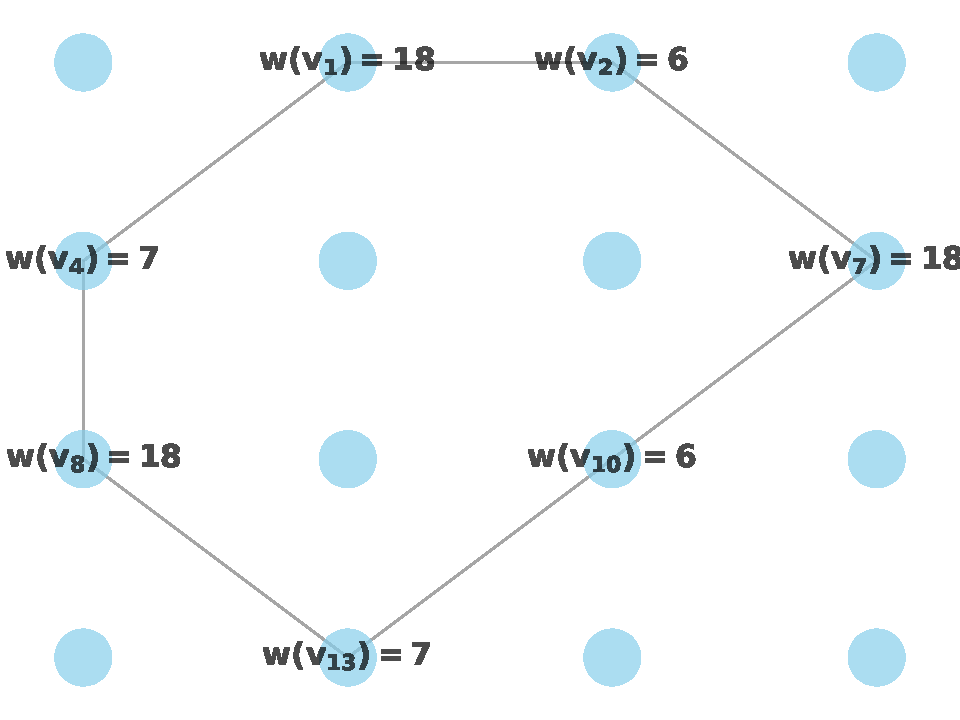
\includegraphics[width=0.8\linewidth]{figures/ICV0.pdf}
    \end{subfigure}
    \hfill
    \begin{subfigure}{0.45\textwidth}
      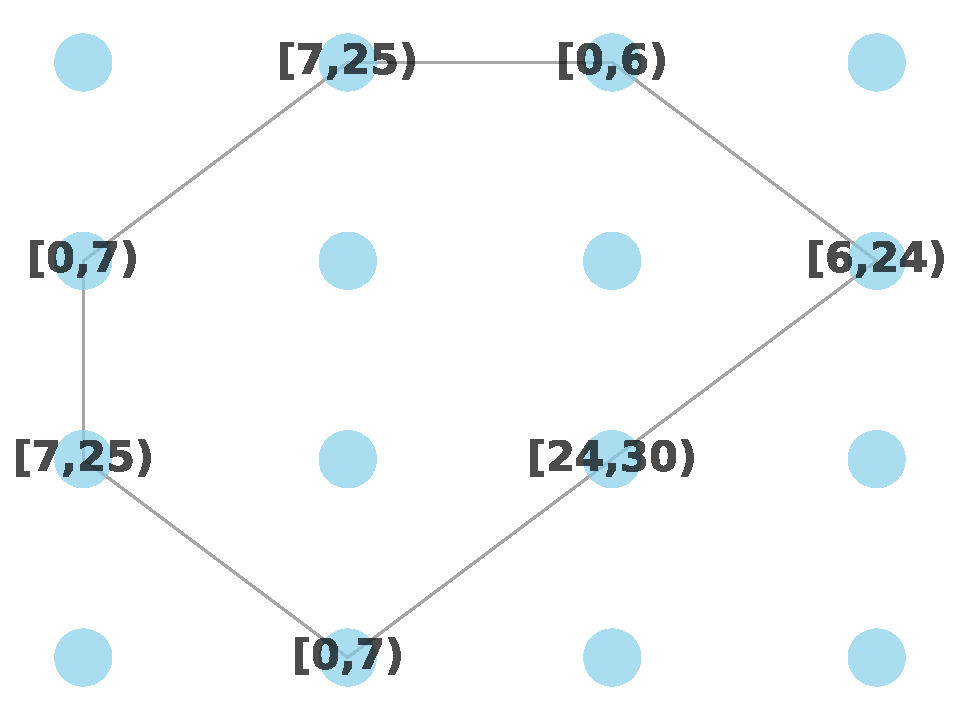
\includegraphics[width=0.8\linewidth]{figures/ICV1.pdf}
    \end{subfigure}
    \hfill
  \end{figure}
  }

\end{frame}